Rețeaua de socializare „GoodCitizen” este formată din două componente: o aplicație web de tipul SPA și 
o aplicație server de tipul REST Web API. Aplicația server folosește o baza de date relațională PostgreSQL. 
Aplicația web este găzduită pe \textit{GoogleFirebase} iar Web API-ul și baza de date pe \textit{Heroku}.

\textit{Heroku} reprezintă o platformă cloud ce suportă diverse limbaje de programare.
\textit{Heroku}, una dintre primele platforme de tip cloud, a fost dezvoltat începând cu anul 2007, când
suporta doar limbajul de programare Ruby, dar de atunci a adăugat suport pentru limbajele Java, 
Python, Node.js, Php și Scala.

\textit{Firebase} este o platformă de dezvoltare pentru aplicații mobile și web. Compania fondatoare a fost înființată în 2011 de 
Andrew Lee și James Tamplin. Proiectul inițial \textit{Firebase} a fost o bază de date în timp real, ce expunea un 
API ce oferea dezvoltatorilor posibilitatea de a stoca și sincroniza datele între mai mulți clienți. 
În timp, și a extins gama de produse pentru a permite dezvoltatorilor un set complet servicii. 
Compania a fost cumpărată de \textit{Google} în octombrie 2014.

Aplicația web poate rula pe ultimele versiuni ale navigatoarelor web: Google Chrome, Mozilla Firefox și Opera. 
Având un design responsive aplicația poate fi accesata și de pe dispozitive mobile.

    Aplicația client este dependentă de cea server, serviciile web expuse de Web API fiind absolut necesare 
pentru funcționarea aplicație.

\section{Funcțiile rețelei de socializare}
În continuare sunt enumerate funcționalitătile aplicației dezvoltate.
\begin{itemize}
    \item{Autentificarea/Înregistrare utilizatorilor:}
        \begin{itemize}
            \item un utilizator nu poate folosi aplicația fără a deține un cont;
            \item autentificarea are rolul de a oferi acces în aplicație utilizatorilor ce au deja un cont;
            \item înregistrarea are scopul de crea un cont pentru noii utilizatori;
        \end{itemize}
    \item{Recuperarea parolei:}
        \begin{itemize}
            \item oferă un serviciu de recuperare a parolei, pentru utilizatorii care și-au uitat parola;
            \item utilizatorii primesc o nouă parola pe adresa de e-mail folosită la înregistrare; 
        \end{itemize}
    \item{Funcționalități de profil:}
        \begin{itemize}
            \item utilizatorii își pot vizualiza datele de profil;
            \item posibilitatea de editare a datelor de profil ;
            \item poza de profil poate fi schimbată la editarea profilului;
        \end{itemize}
    \item{Crearea unei comunități:}
        \begin{itemize}
            \item utilizatorii au posibilitatea de a crea comunități;
            \item posibilitatea de editare a unei comunități este disponibilă doar creatorului
            comunității;
            \item creatorul comunității poate adăuga noi realizări;
            \item funcționalitatea de a adăuga administratori în comunitate îi este disponibilă doar creatorului;
        \end{itemize}
    \item{Administrarea comunității:}
        \begin{itemize}
            \item un administrator are dreptul de a adăuga și edita realizări;
            \item administratorul nu are dreptul de editare a datelor de profil ale comunității; 
        \end{itemize}
    \item{Interacțiunile în comunitate:}
        \begin{itemize}
            \item scopul unei comunități este de grupa și adaugă realizări în aplicație;
            \item un utilizator se poate alătura unei comunități;
            \item un utilizator poate părăsi o comunitate fără a pierde realizările câștigate;
            \item posibilitatea de căutare membrilor unei comunități;
            \item căutarea unei realizări câștigate de membrii comunității;
            \item căutarea unei realizări specifice unei comunități;
        \end{itemize}
    \item{Interacțiunile între utilizatori:}
        \begin{itemize}
            \item utilizatorii pot urmări alți membri pentru a putea fi la curent cu realizările acestora;
        \end{itemize}
    \item{Tipuri de realizări disponibile pentru utilizator:}
        \begin{itemize}
            \item utilizatorii au la dispoziție un set de realizări globale pe care le pot încerca;
            \item realizările din comunități pot fi încercate doar dacă utilizatorul este membru;
        \end{itemize}
    \item{Funcționalități orientate pe realizările proprii unui utilizator:}
        \begin{itemize}
            \item vizualizarea realizărilor câștigate;
            \item vizualizarea realizărilor în curs de apreciere;
            \item stergerea unei realizări în curs de apreciere;
        \end{itemize}  
    \item{Funcționalități orientate pe realizările utilizatorilor:} 
        \begin{itemize}
            \item vizualizarea realizărilor câștigate/în curs de apreciere a realizărilor utilizatorilor;
            \item posibilitatea de a aprecia realizările altor utilizatori;
            \item în cazul în care un utilizator consideră ca o realizare în curs de apreciere a unui utilizator este 
            falsă, necorespunzătoare sau cu un conținut vulgar, accesa poate marca realizarea ca fiind defectuoasă;
            \item posibilitatea de a vedea realizările adăugate în apropriere ce sunt câștigate sau în curs de apreciere;
        \end{itemize}  
    \item{Modalitatea de premiere a utilizatorilor:} 
        \begin{itemize}
            \item fiecare realizare are un număr specific de puncte;
            \item o realizare în curs de apreciere are nevoie de un număr specific aprecieri pentru a trece în
            stadiul de „câștigat”;
            \item numărul de puncte câștigate de un utilizator sunt adunate și afișate pe propriul profil;
        \end{itemize}  
\end{itemize}


În continuare sunt prezentate în detaliu funcționalitățile sistemului.Totodată este prezentat 
și sistemul de premiere a utilizatorilor. Pentru prezentarea mai explicită vor fi adăugate imagini reprezentative. 
Imaginile reprezintă capturi de ecran alea rețelei de socializare pe diferite dispozitive, astfel evidențiindu-se designul responsive.  
\subsection{Înregistrarea și autentificarea în aplicație} 
 
    Pentru a putea folosi rețeaua de socializare „GoodCitizen”, un utilizator trebui mai întâi să se înregistreze. Datele de  
    înregistrare necesare sunt: username, nume, prenume, e-mail și parolă (Fig.~\ref{fig:login}). Username-ul și adresa de e-mail-ul trebuie  
    să fie unice, astfel în cazul în care un utilizator încearcă sa folosească date deja folosite, acesta  
    va primi mesaje de eroare. Înregistrarea este prevăzută și cu un sistem de verificare a parolei  
    ce consta în doua câmpuri pentru parolă. Acest sistem verifică dacă parolele din cele două câmpuri corespund.  
    Acest sistem este util în cazul în care utilizatorul introduce parola greșit.În cazul în care utilizatorul 
    are deja un cont, acesta se poate autentifica direct. Dacă contul este creat cu succes, noul utilizator va primi un e-mail cu  
    un mesaj de bun venit. 
    \begin{figure}[h] 
    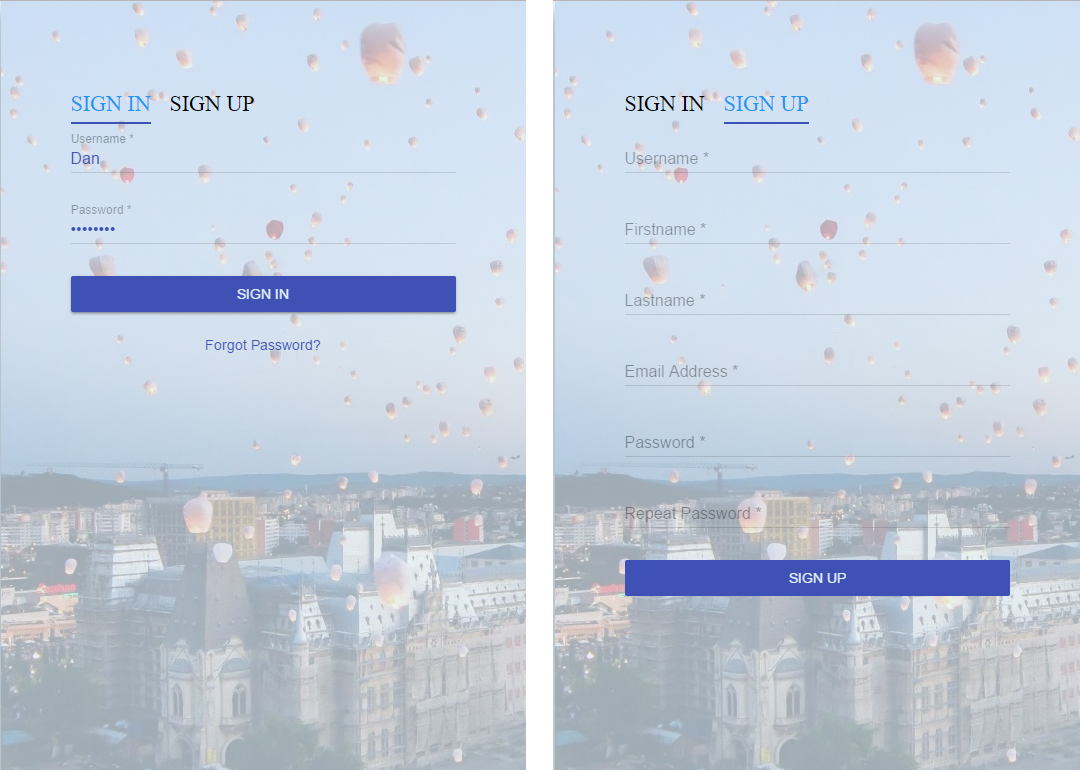
\includegraphics[height=0.6\linewidth]{login.png} 
    \centering 
    \caption{Autentificarea și înregistrarea în aplicație.} 
    \label{fig:login} 
    \end{figure}  
 
    Pentru autentificarea în aplicație, utilizatorul are nevoie să își cunoască username-ul sau adresa e-mail și parola. 
\subsection{Resetarea parolei} 

    În cazul în care utilizatorul își pierde parola acesta își poate reseta parola introducând adresa de e-mail (Fig.~\ref{fig:reset-password}).
    Dacă utilizatorul își uită adresa de e-mail acesta nu își va mai putea recupera contul.
    Utilizatorul va primi pe adresa de e-mail introdusă o nouă parolă generată aleatoriu(Fig.~\ref{fig:email}).
    \begin{figure}[h]
    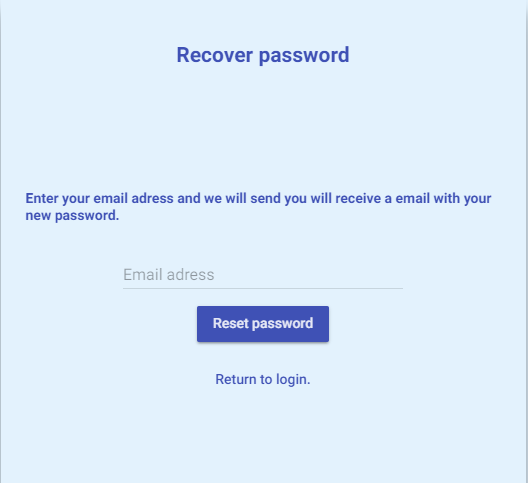
\includegraphics[height=0.6\linewidth]{reset-password.png}
    \centering
    \caption{Resetarea parolei}
    \label{fig:reset-password}
    \end{figure} 
    \begin{figure}[h]
    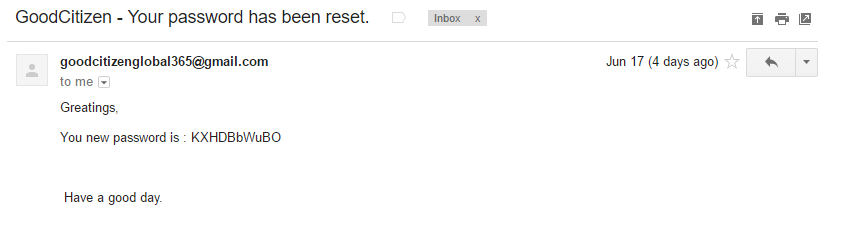
\includegraphics[height=0.25\linewidth]{email.png}
    \centering
    \caption{Conținutul unui e-mail de resetarea a parolei.}
    \label{fig:email}
    \end{figure}
\subsection{Ce sunt realizările?}

    Realizările reprezintă unitatea de bază a rețelei de socializare. Toate funcționalitătile rețelei de socializare sunt modalități de 
    descoperire și câștigare a realizărilor. în capitolele următoare vor fi prezentate aceste funcționalități.
    
    Utilizatorii aplicației au la dispoziție o lista de realizări globale pe care aceștia le pot încerca (Fig.~\ref{fig:global-achievements}). 
    Acestea pot fi filtrate în funcție de categorie sau căutate după nume sau descriere. 
    \begin{figure}[h]
    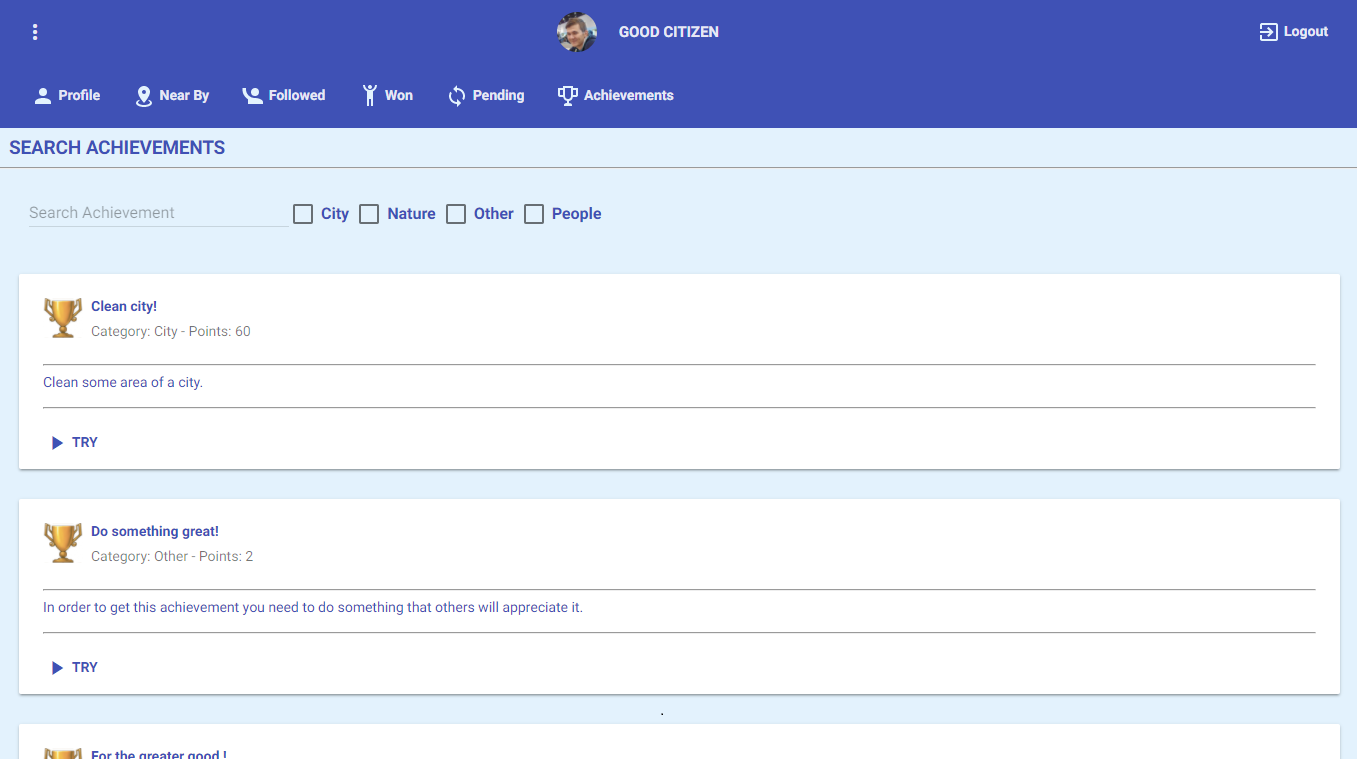
\includegraphics[width=\textwidth,height=\textheight,keepaspectratio]{global-achievements.png}
    % 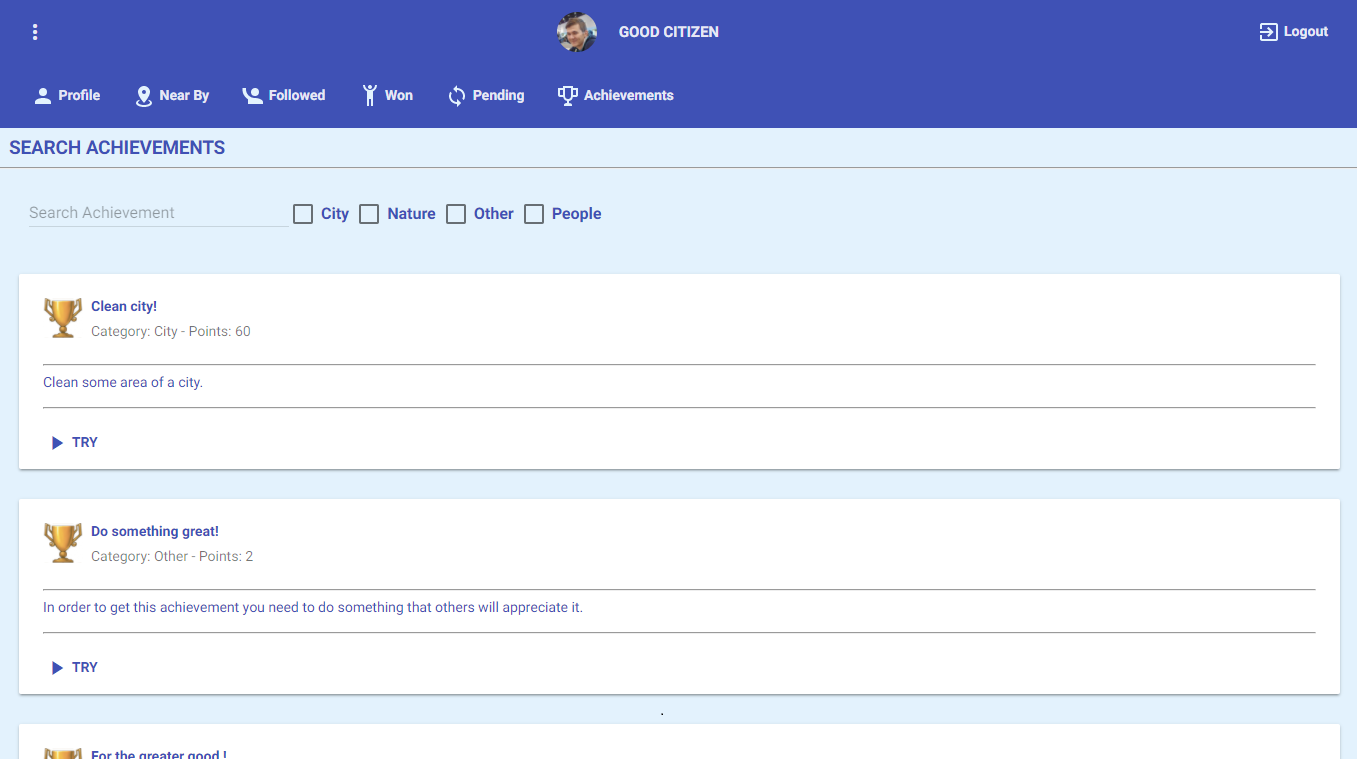
\includegraphics[height=0.58\linewidth]{global-achievements.png}
    \centering
    \caption{Lista de realizări globale.}
    \label{fig:global-achievements}
    \end{figure}
\subsubsection{Procesul de încercarea unei realizări}

    Încercarea unei realizări reprezintă procesul prin care un utilizator publică o realizare de a sa 
    pentru a fi văzută de alți cetățeni. Pentru a încerca o realizare utilizatorii trebuie să adauge o fotografie 
    proprie drept dovadă și o descriere scurtă a gestului lor benefic societății.
    Utilizatorul poate introduce locația în care a avut loc fapta sa. Orice realizare încercată trebuie să aibă o locație. 
    În mod standard locația este este setată prin intermediul serviciului de geolocatie, însa utilizatorul 
    are și posibilitatea de a seta o locatie (Fig.~\ref{fig:achievement-add}).

    \begin{figure}[h]
    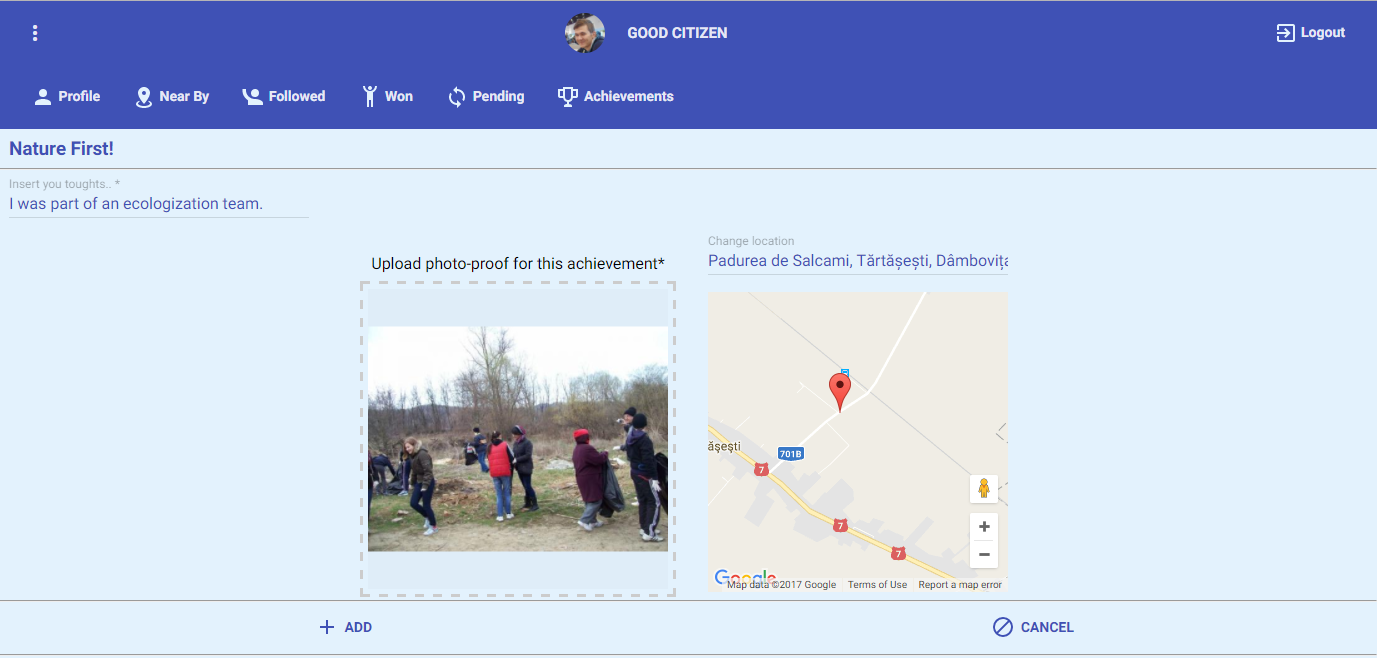
\includegraphics[width=\textwidth,height=\textheight,keepaspectratio]{achievement-add.png}
    % 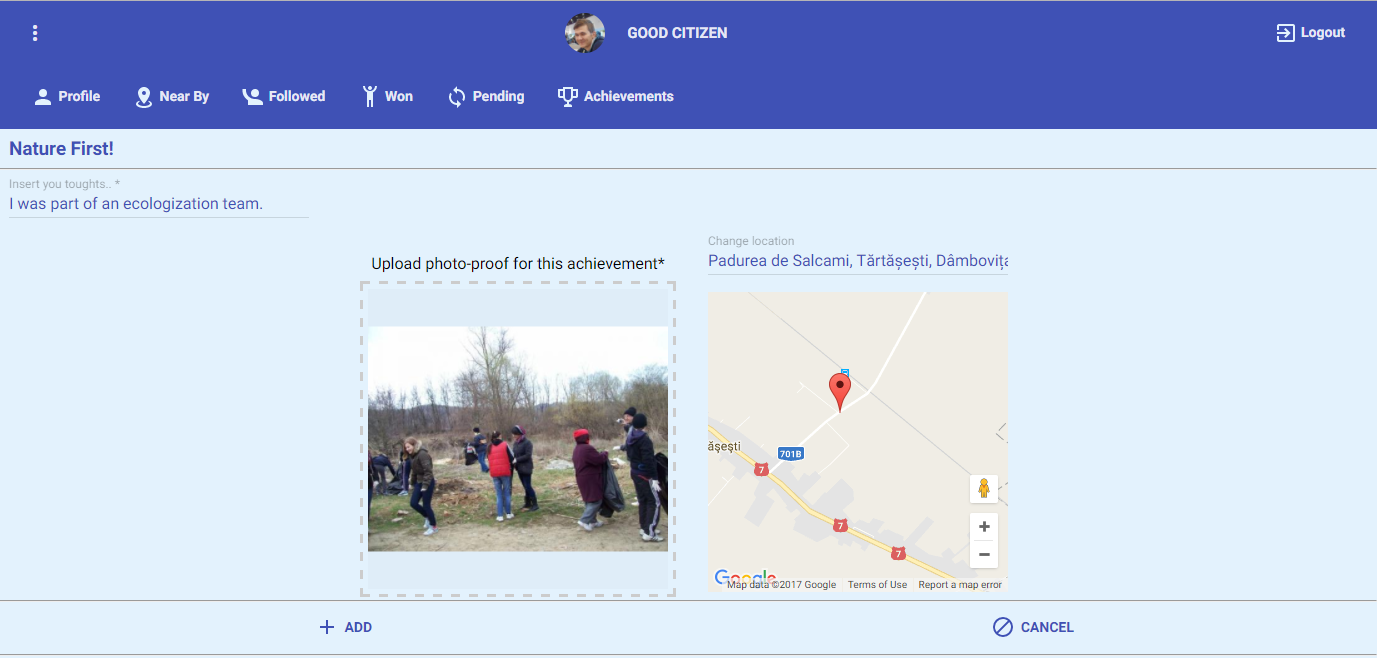
\includegraphics[height=0.5\linewidth]{achievement-add.png}
    \centering
    \caption{Încercarea unei realizări.}
    \label{fig:achievement-add}
    \end{figure} 
\clearpage
\subsubsection{Vizualizarea realizărilor proprii}

    Utilizatori își pot vizualiza propriile realizări. Acestea sunt afișate pe paginile „Won” și „Pending”.
    O realizare proprie aflată în procesul de apreciere poate fi ștearsă folosind butonul „CANCEL” (Fig.~\ref{fig:achievement-pending}) de pe pagina 
    „Pending”. Utilizatorul nu este penalizat pentru ștergerea unei realizări.
    \begin{figure}[h]
    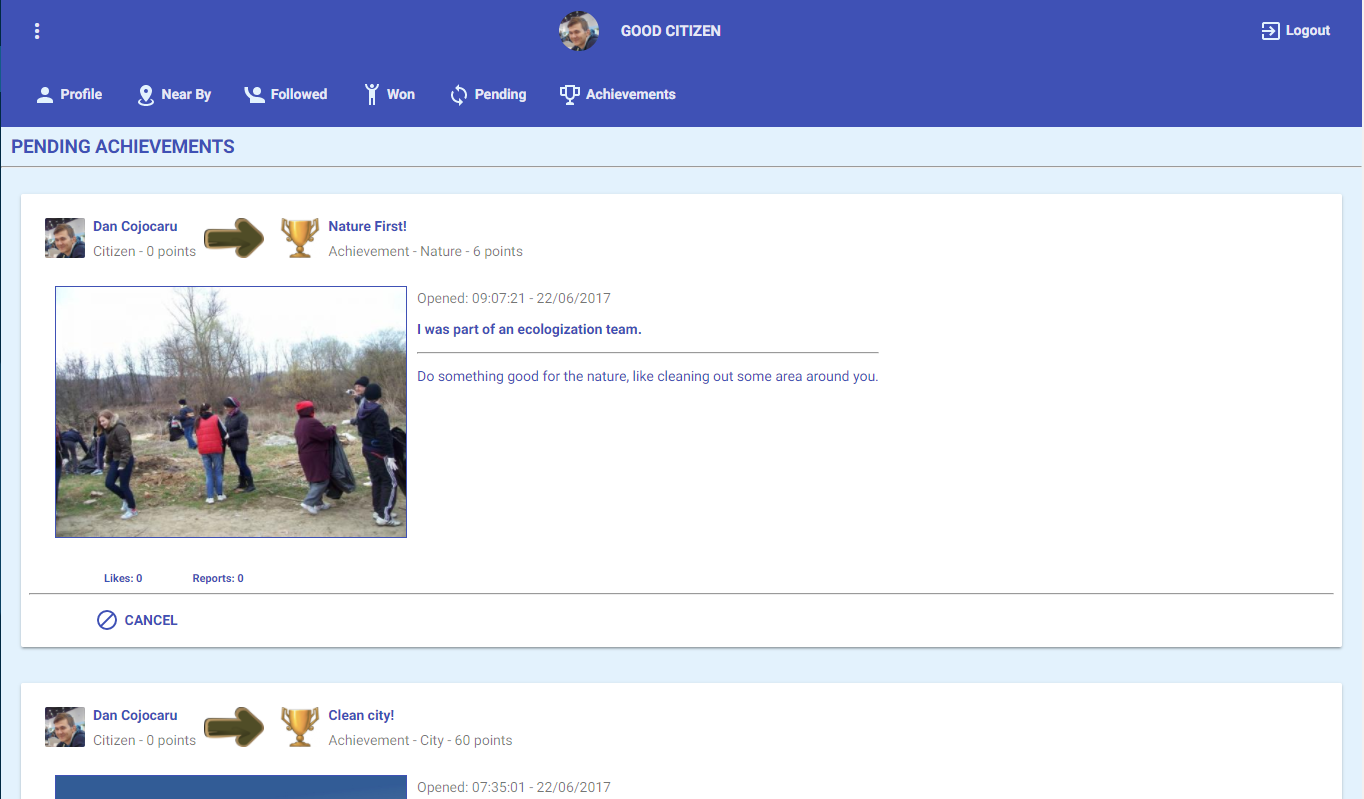
\includegraphics[width=\textwidth,height=\textheight,keepaspectratio]{achievement-pending.png}
    % 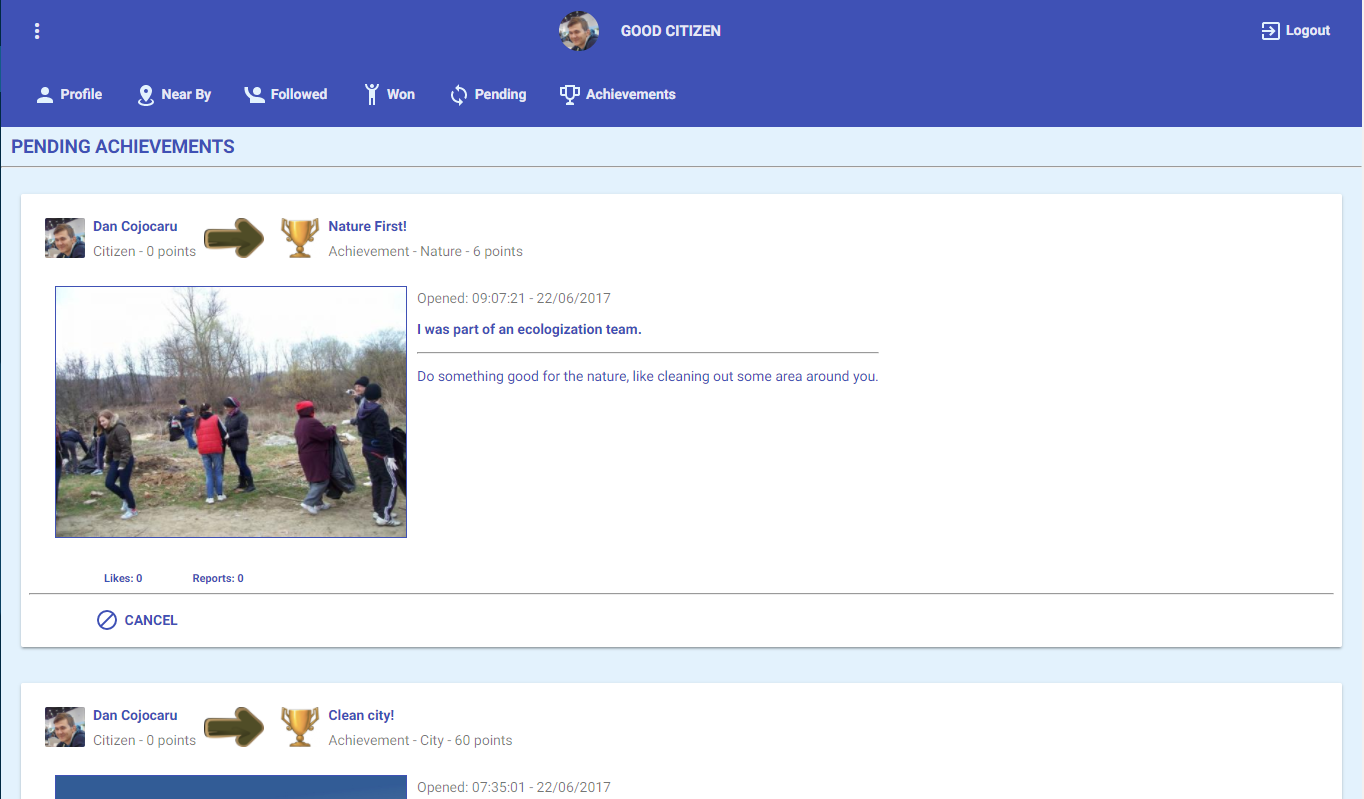
\includegraphics[height=0.6\linewidth]{achievement-pending.png}
    \centering
    \caption{Realizări în curs de apreciere.}
    \label{fig:achievement-pending}
    \end{figure} 

\subsubsection{Procesul de votare a realizărilor în curs de apreciere}

    Realizările în curs de apreciere sunt reprezentate de realizările pe care utilizatorii încearcă să le câștige.

    Utilizatori au la dispoziție două alegeri în procesul de apreciere/votare. Aceștia pot da „Like”, dacă 
    consideră că realizarea este corespunzătoare cu descrierea, sau „Report” dacă dovezile adăugate de utilizator 
    nu sunt convingătoare, nu coincid descrierii sau au un conținut vulgar. Orice vot eronat poate fi anulat.
    Fiecare realizare are un număr specific de like-uri necesare pentru a fi câștigată. 
    Realizările cu 50 de voturi negative(„Report”) sunt considerate neadecvate și sunt șterse. 
    Utilizatorul ce a adăugat realizarea neadecvată va primi o penalizare în puncte echivalentă cu numărul de puncte 
    ale realizării.

    Realizările câștigate sau în curs de apreciere ale altor utilizatori pot fi vizualizate pe paginile 
    „Followed”(Fig.~\ref{fig:followed-pending}) și „NearBy”(Fig.~\ref{fig:nearby}). Pe pagina „Near By” sunt vizibile realizările 
    utilizatorilor din apropriere. Utilizatorul pote sorta realizările în funcție de raza(în kilometri) pe care aceștia o setează. 
    Raza setată reprezintă raza unui cerc ce are centrul în poziția actuală a utilizatorului. Această funcționalitate este 
    disponibilă doar dacă este activ serviciul de geolocație de pe dispozitivul folosit.
    Pentru vizualiza realizările câștigate de cetățenii urmăriți, utilizatorul trebuie să folosească 
    butonul „display won achievements”(Fig.~\ref{fig:followed-pending}).
    \begin{figure}[h]
    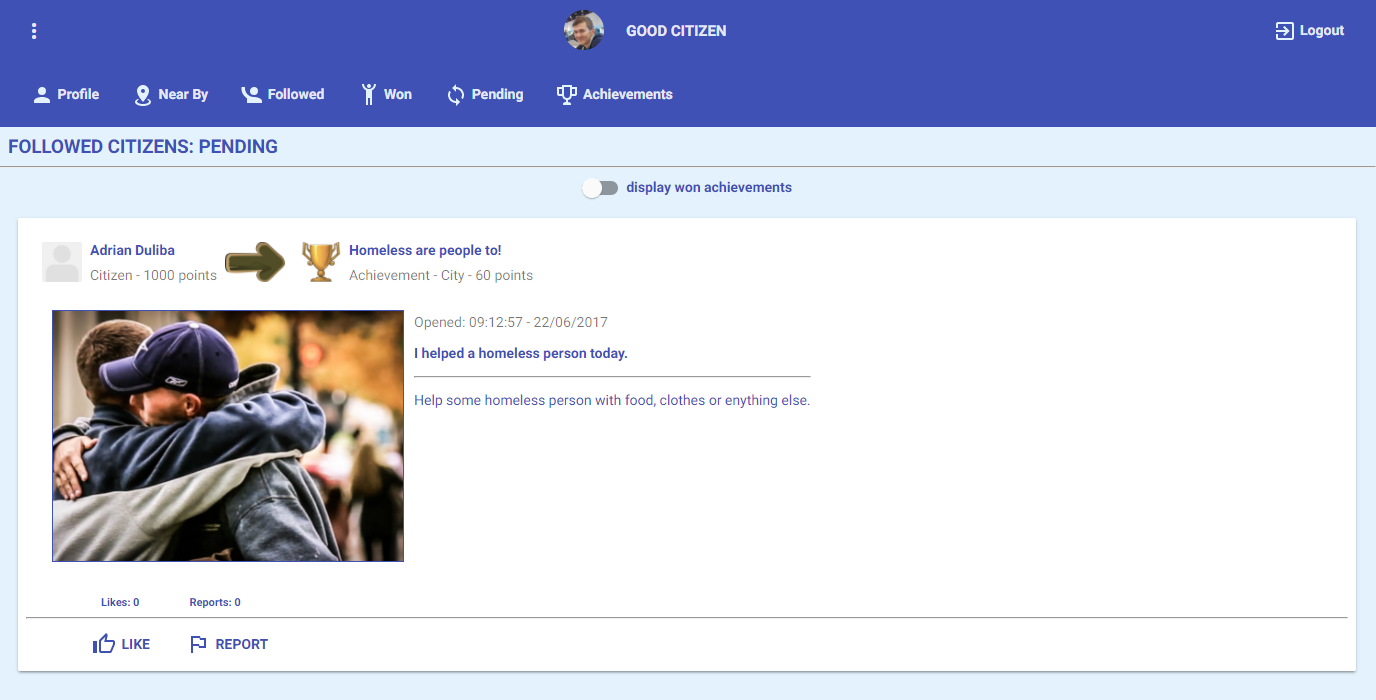
\includegraphics[width=\textwidth,height=\textheight,keepaspectratio]{followed-pending.png}
    % 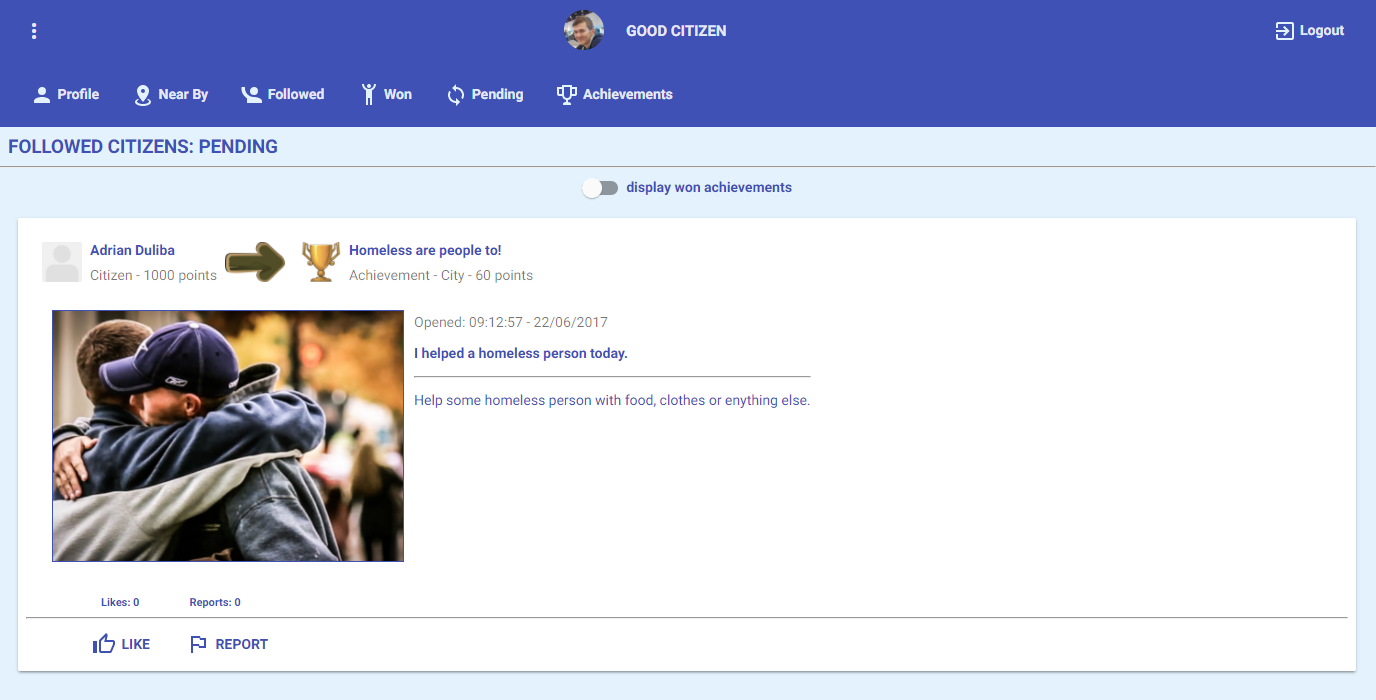
\includegraphics[height=0.53\linewidth]{followed-pending.png}
    \centering
    \caption{Realizările îndeplinite/în curs de apreciere ale cetățenilor urmăriți.}
    \label{fig:followed-pending}
    \end{figure} 
    \begin{figure}[h]
    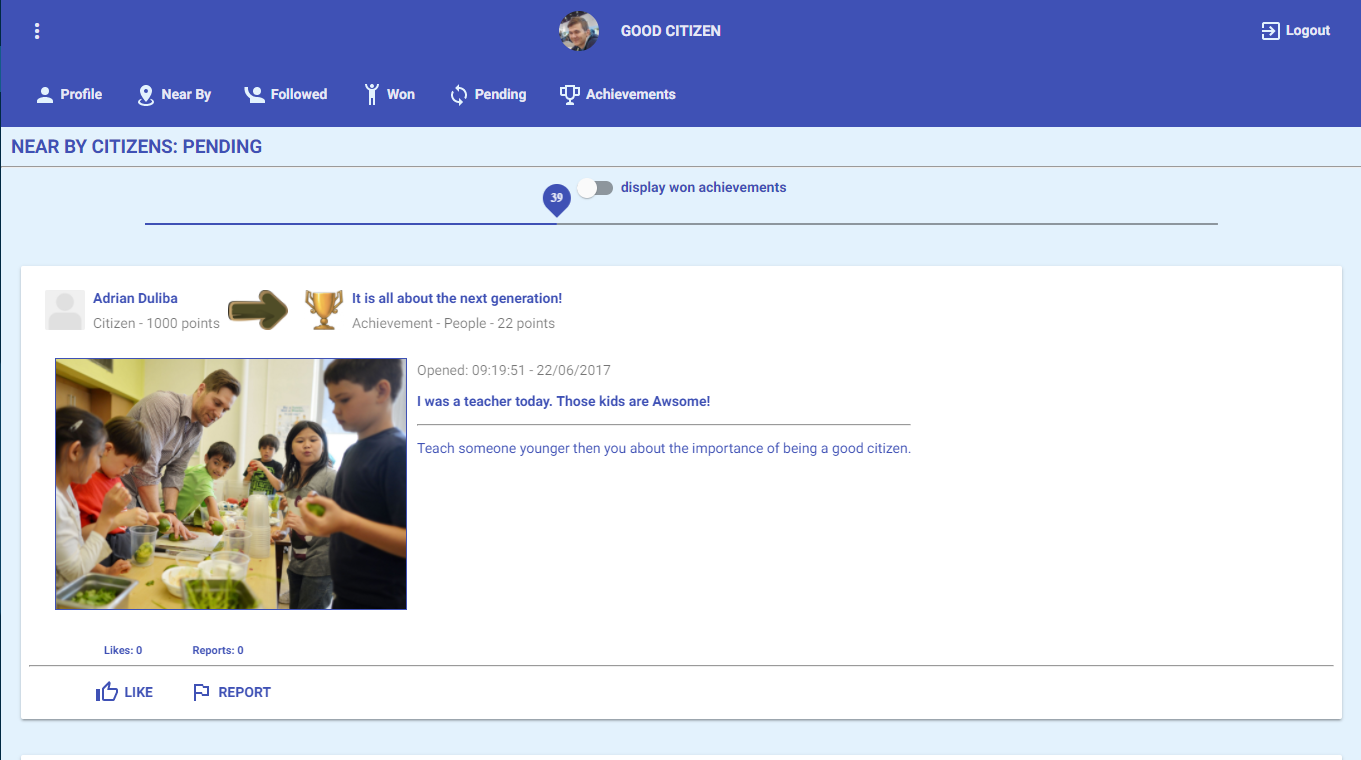
\includegraphics[width=\textwidth,height=\textheight,keepaspectratio]{nearby.png}
    % 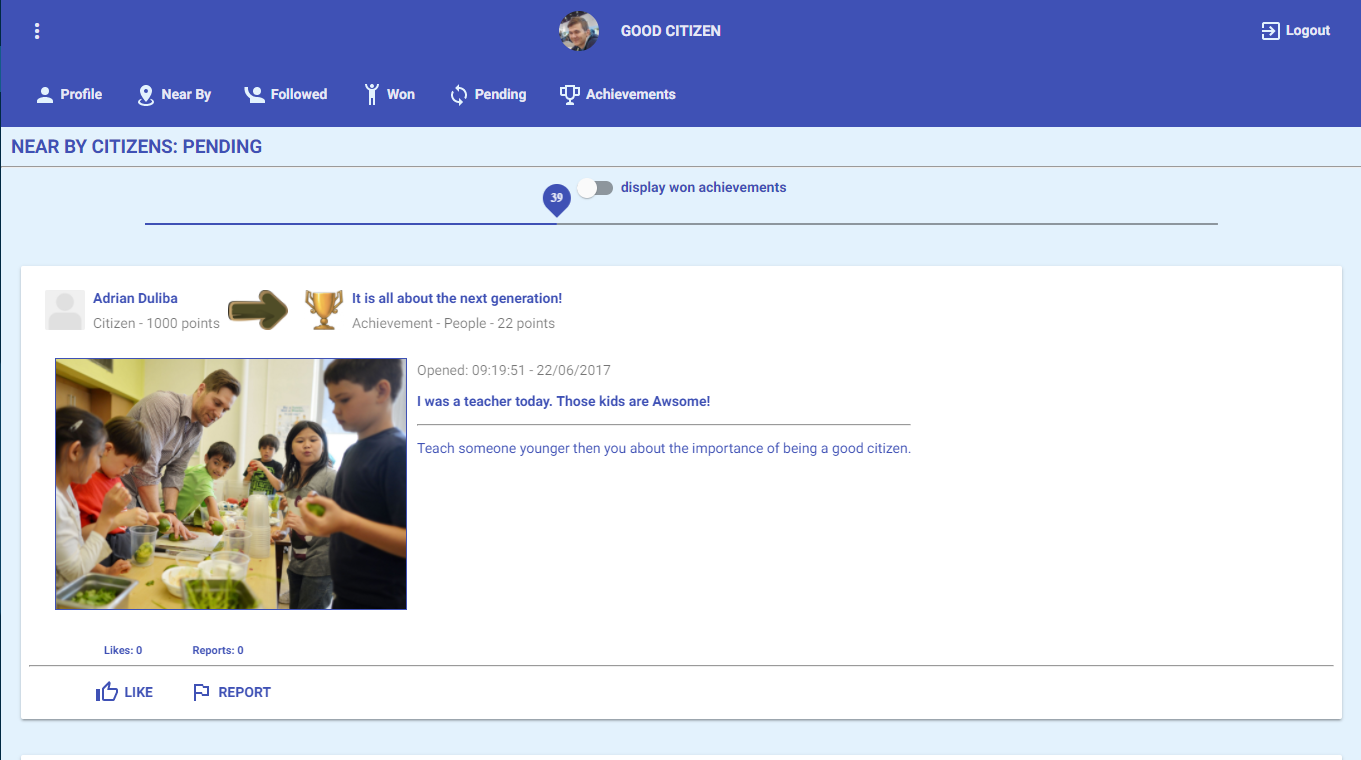
\includegraphics[height=0.58\linewidth]{nearby.png}
    \centering
    \caption{Realizările îndeplinite/în curs de apreciere ale cetățenilor din apropiere.}
    \label{fig:nearby}
    \end{figure} 
\pagebreak
\subsection{Profilul cetățeanului}

    Profilul reprezintă imaginea virtuală pentru fiecare cetățean în aplicație (Fig.~\ref{fig:profile}). Paginile de profil
    sunt publice oricărui utilizator din aplicație deoarece într-o aplicație în care sunt promovate faptele bune nu
    ar trebui să fie nimic ascuns, cu excepția adresei de e-mail și a parolei.

    Pagina de profil conține legăturile care alte pagini cum ar fi: utilizatori urmăriți, utilizatori ce urmăresc profilul curent, 
    comunitățile de care aparține utilizatorul și editarea profilului.

    Profilul conține informații legate de activitatea utilizatorului: numărul de urmăritori, 
    numărul de utilizatori urmăriți, numărul de comunități, numărul de puncte câștigate și un grafic ce prezintă activitatea 
    utilizatorului în ultimele 7 zile. Graficul cu statistici prezintă numărul de puncte câștigate pe zi și numărul 
    de puncte pierdute pe zi.
    \begin{figure}[h]
    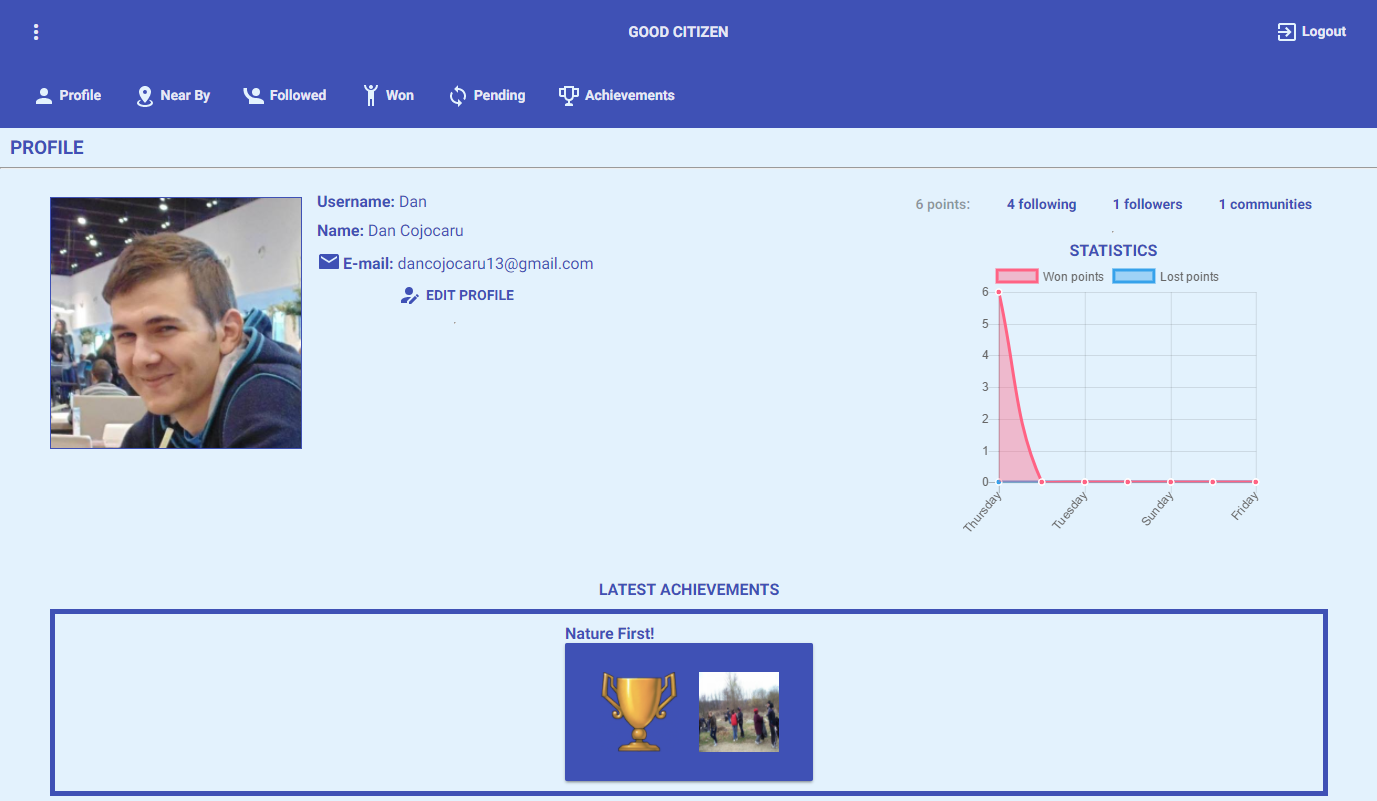
\includegraphics[width=\textwidth,height=\textheight,keepaspectratio]{profile.png}
    % 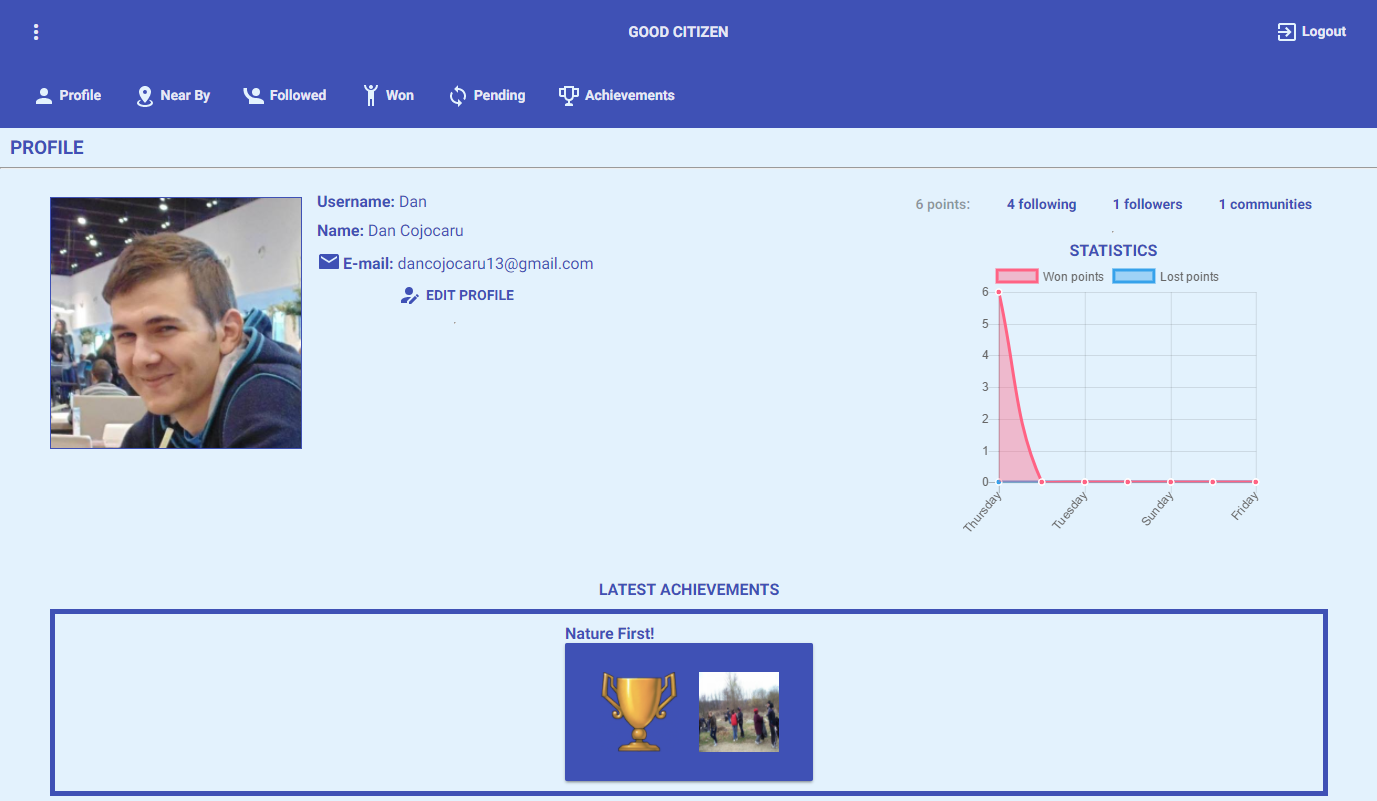
\includegraphics[height=0.6\linewidth]{profile.png}
    \centering
    \caption{Profilul utilizatorului.}
    \label{fig:profile}
    \end{figure} 
\subsubsection{Editarea datelor personale}

    Utilizatorul are posibilitatea de a-și modifica datele de profil (Fig.~\ref{fig:edit-profile}). Acesta își poate schimba numele, prenumele, adresa de e-mail, 
    și parola. De asemenea utilizatorul își poate modifica și poza de profil. Dacă poza de profil nu există, utilizatorul va avea
    ca poza de profil o imagine standard.
    \begin{figure}[h]
    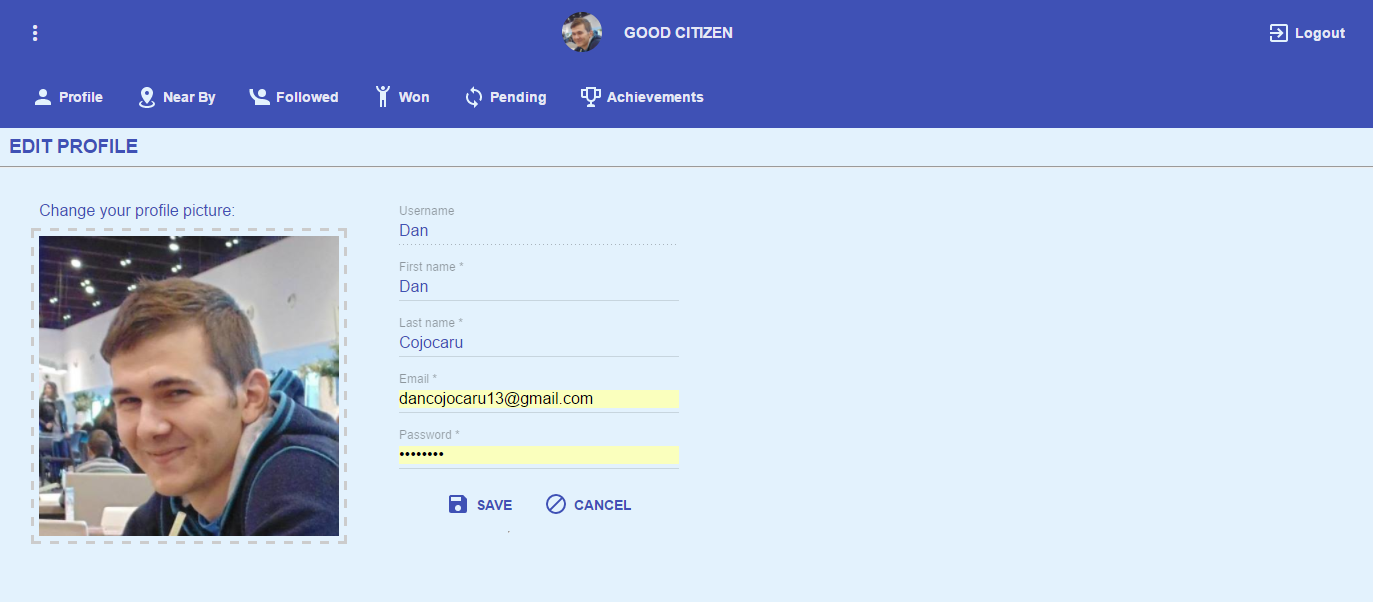
\includegraphics[width=\textwidth,height=\textheight,keepaspectratio]{edit-profile.png}
    % 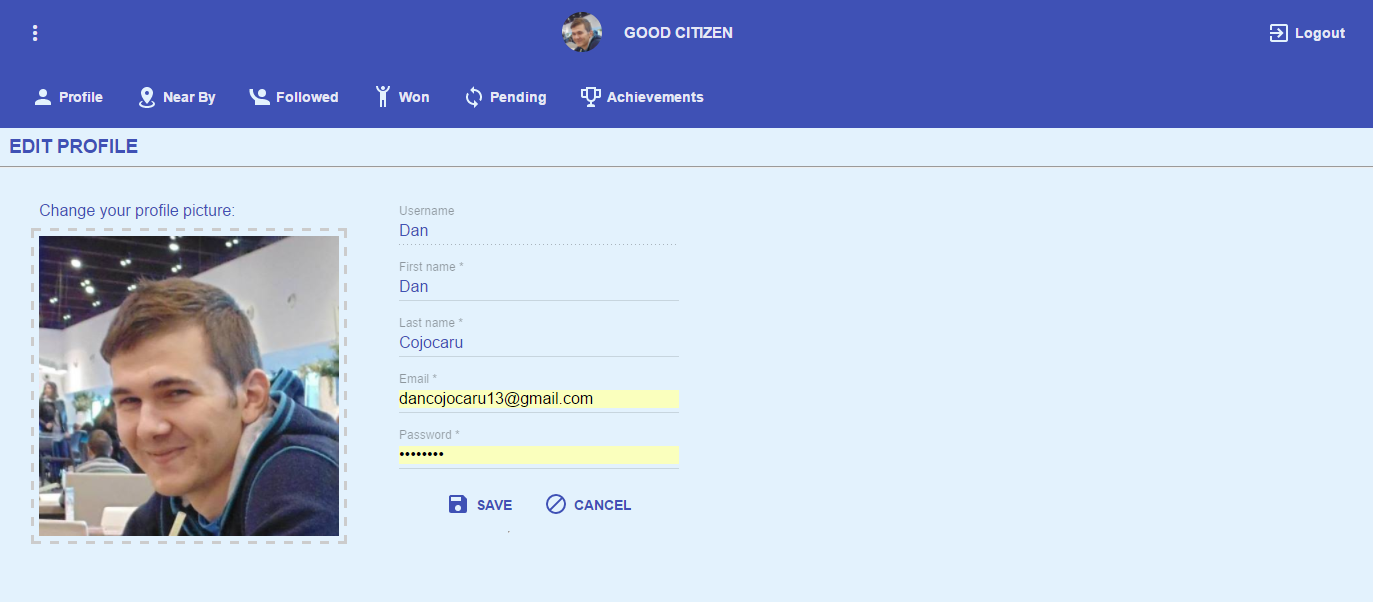
\includegraphics[height=0.45\linewidth]{edit-profile.png}
    \centering
    \caption{Editarea profilului.}
    \label{fig:edit-profile}
    \end{figure} 

\subsection{Stabilirea relațiilor dintre cetățeni}
    
    Utilizatorii pot căuta cetățeni și comunități în aplicație prin intermediul modalităților de căutare, 
    așa cum sunt prezentate în figura Fig.~\ref{fig:find}. Navigarea către profilul unui utilizator este posibilă
    de pe fiecare apariție a cetățeanului într-o realizare (Fig.~\ref{fig:community-pending}).

    Relațiile dintre cetățeni se pot stabili și prin intermediul comunităților. 
    \begin{figure}[h]
    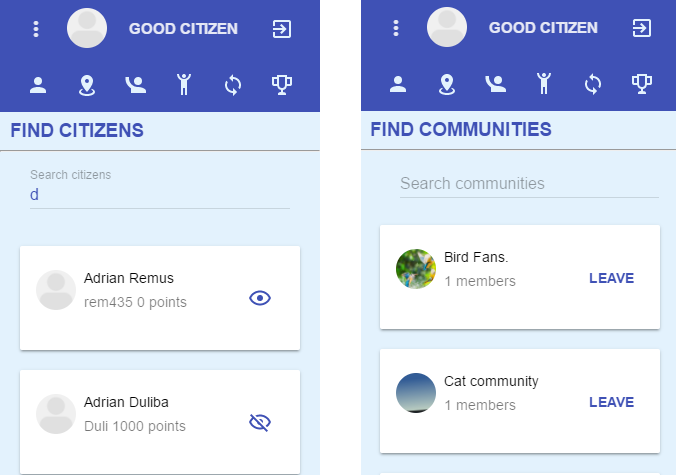
\includegraphics[height=0.6\linewidth]{find.png}
    \centering
    \caption{Căutarea comunităților și cetățenilor în rețeaua de socializare.}
    \label{fig:find}
    \end{figure}   
\subsubsection{Ce sunt comunitățile ?}

    O comunitate reprezintă o modalitate de a crea relații între utilizatori cu aceeași viziune,
    asupra unei comunități din viața reală sau virtuală. O comunitate are rolul de a oferi 
    utilizatorului posibilitatea de a vizualiza realizări ale altor cetățeni cu idealuri și 
    mentalități asemănătoare. Comunitățile pot fi bazate pe oameni din aceleași 
    zone geografice(orașe, județe, țări, regiuni, etc). De exemplu un cetățean se poate 
    alătura unei comunități ce aparține orașului în care locuiește pentru a putea câștiga 
    realizări specifice acelui oraș. Astfel comunitatea reprezintă și o modalitate de gruparea 
    a realizărilor pe orașe, ideologii, interese comune, etc.

    Utilizatorii pot deveni membrii sau pot părăsi o comunitate oricând doresc fără 
    a le afecta progresul în rețeaua de socializare. Aceștia pot vizualiza comunității, realizări ale 
    membrilor și realizări posibile în cadrul comunității (Fig.~\ref{fig:community-achievements}) .

    Creatorul unei comunități poate oferi drepturi de administrator oricărui membru (Fig.~\ref{fig:community-profile}).
  
    Atribuțiile unui administrator sunt de a adăuga și edita realizări pentru comunitate (Fig.~\ref{fig:achievement}).
    O realizare trebuie să aibă: titlu, descriere, categorie, numărul necesar de like-uri pentru a fi câștiga,
    numărul de puncte și o imagine reprezentativă. 
    \begin{figure}[h]
    % 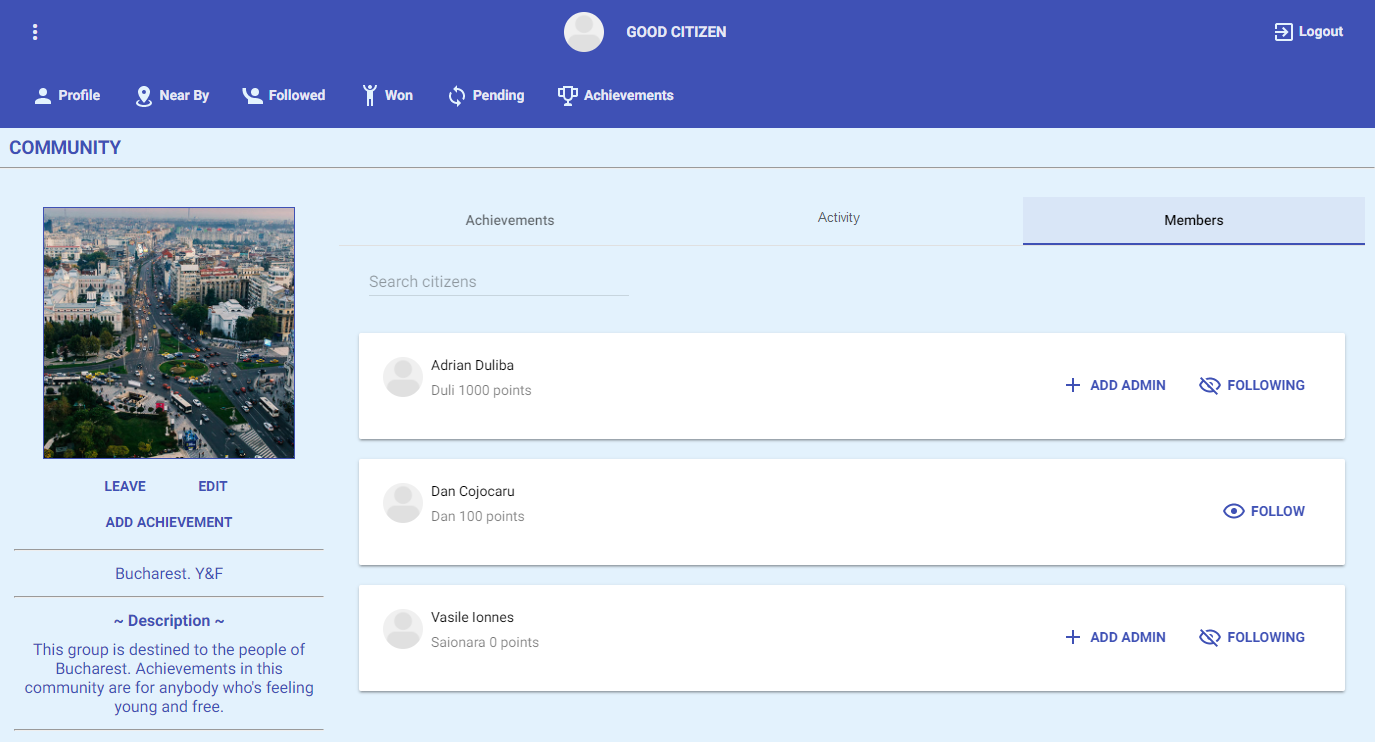
\includegraphics[height=0.55\linewidth]{community-profile.png}
    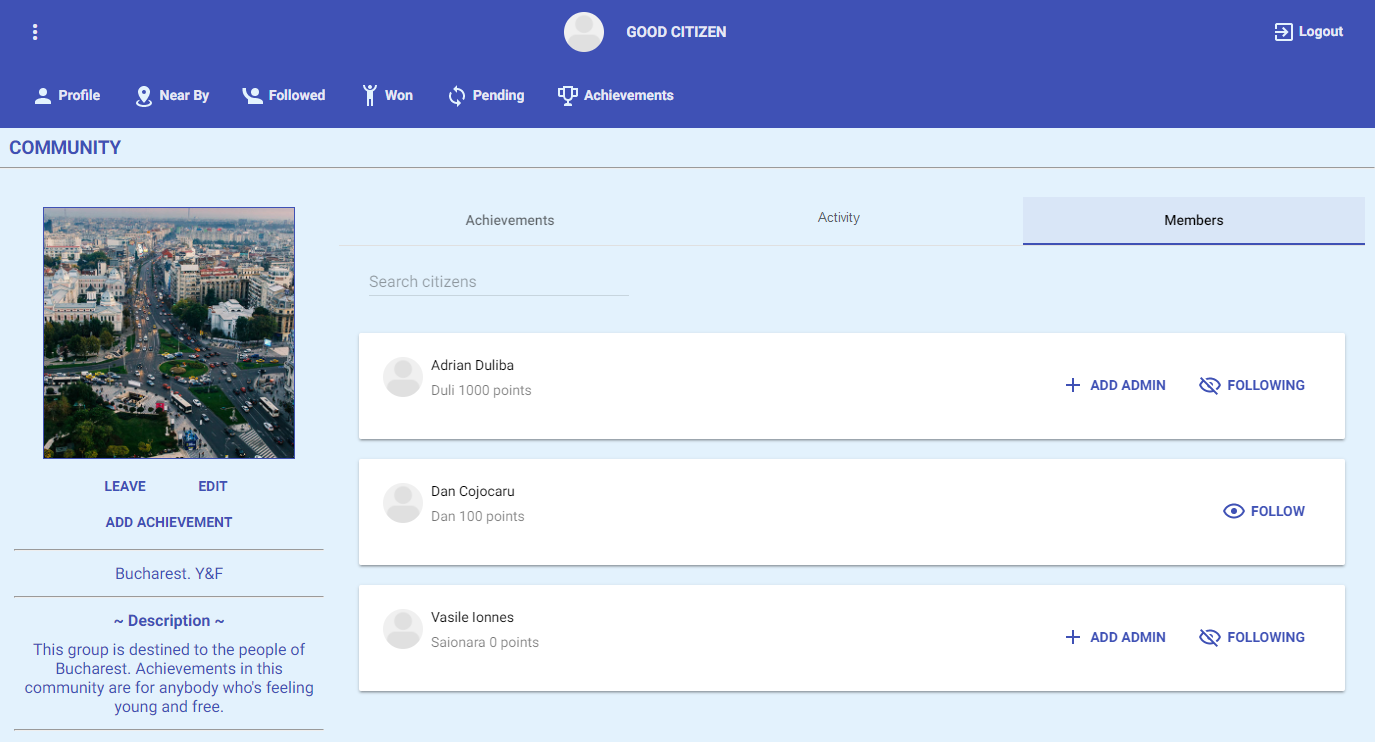
\includegraphics[width=\textwidth,height=\textheight,keepaspectratio]{community-profile.png}
    \centering
    \caption{Profilul unei comunități cu drepturi de creator.}
    \label{fig:community-profile}
    \end{figure}   
    \begin{figure}[h]
    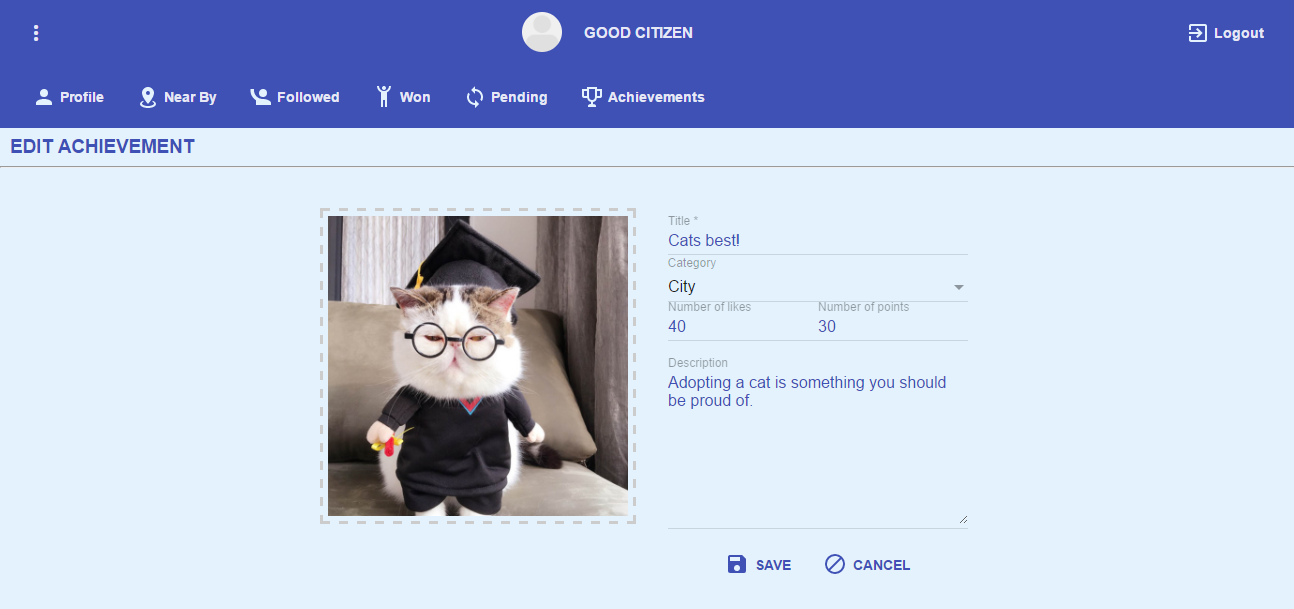
\includegraphics[width=\textwidth,height=\textheight,keepaspectratio]{achievement.png}
    % 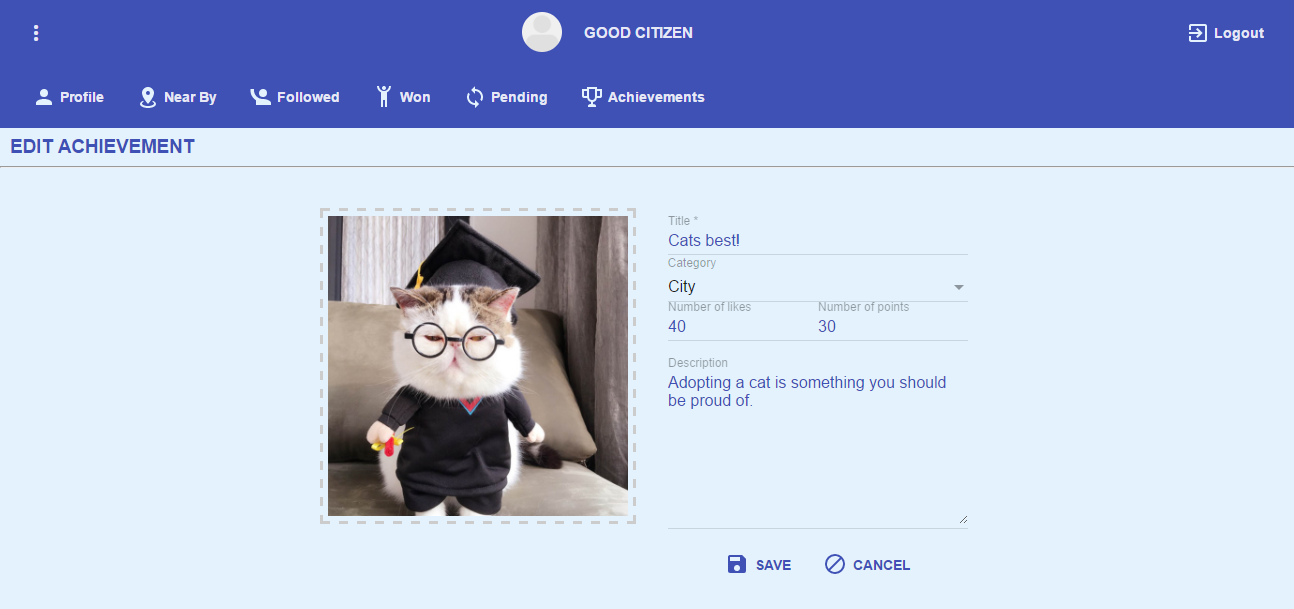
\includegraphics[height=0.48\linewidth]{achievement.png}
    \centering
    \caption{Administrarea unei realizări.}
    \label{fig:achievement}
    \end{figure}  
    \begin{figure}[h]
    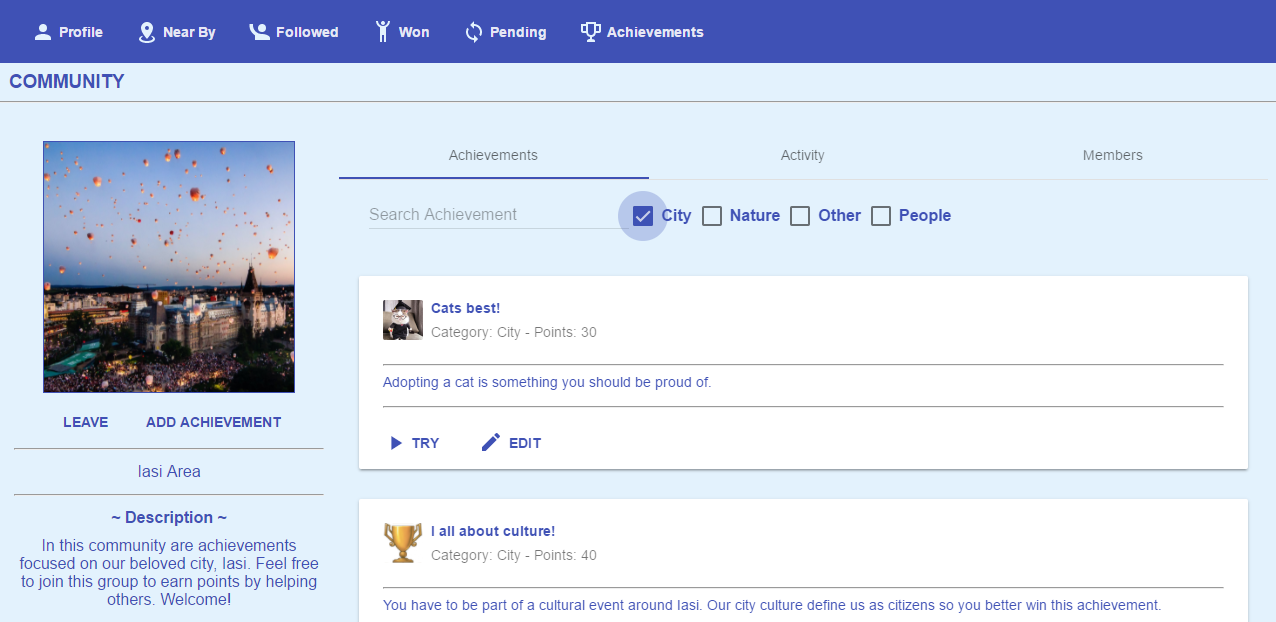
\includegraphics[width=\textwidth,height=\textheight,keepaspectratio]{community-achievements.png}
    % 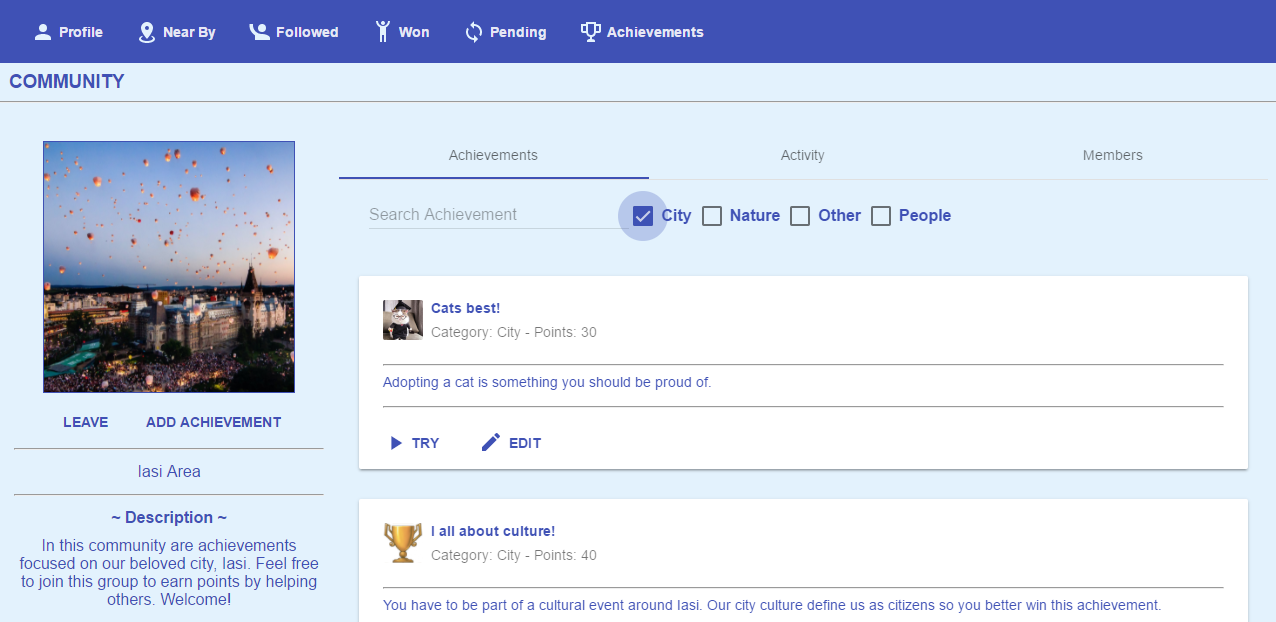
\includegraphics[height=0.50\linewidth]{community-achievements.png}
    \centering
    \caption{Realizările posibile într-o comunitate.}
    \label{fig:community-achievements}
    \end{figure}
    \begin{figure}[h]
    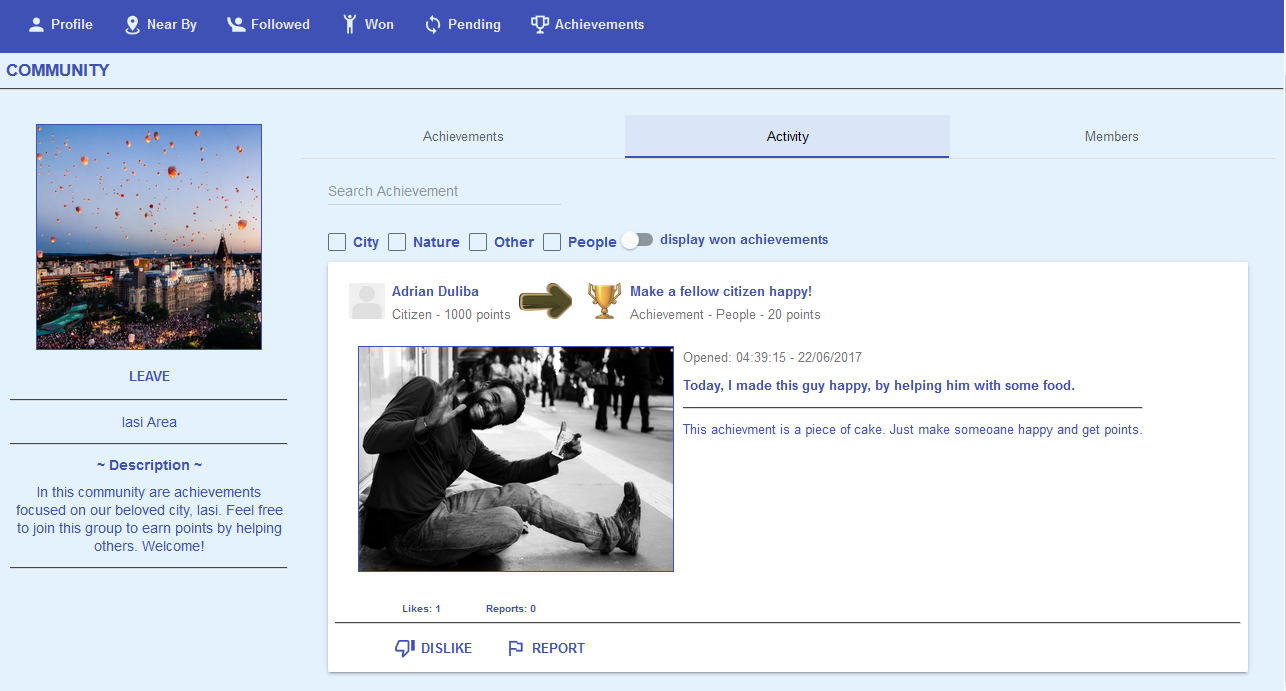
\includegraphics[width=\textwidth,height=\textheight,keepaspectratio]{community-pending.png}
    % 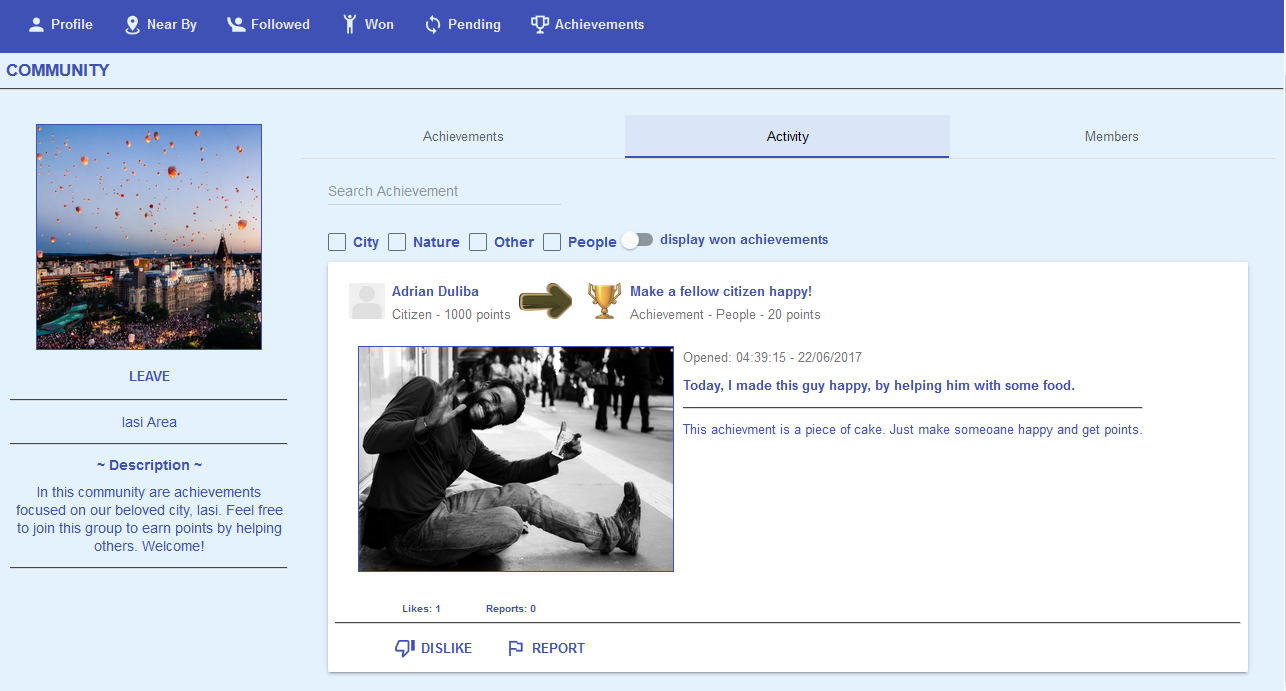
\includegraphics[height=0.55\linewidth]{community-pending.png}
    \centering
    \caption{Activitatea membrilor într-o comunitate.}
    \label{fig:community-pending}
    \end{figure}   
    \clearpage
    \subsubsection{Crearea unei comunități}
    Crearea comunități poate fi realizată de orice utilizator autentificat. Pentru a crea o comunitate 
    trebuiesc introduse: titlul, descrierea și o fotografie ce reprezintă comunitatea. 
    Titlul comunității trebuie sa fie unic în aplicație. Adăugarea unei fotografii nu este obligatorie.
    Titlul și descrierea trebuie fie cât mai specifice astfel încât comunitatea să atragă cați mai mulți 
    cetățeni (Fig.~\ref{fig:create-community}).
    Odată cu crearea unei noi comunități, creatorul devine automat membru al comunității.
    Datele de profil ale comunității pot fi modificate doar de creator. Creatorul reprezintă utilizatorul 
    cu cele mai multe drepturi în comunitate.
    \begin{figure}[h]
    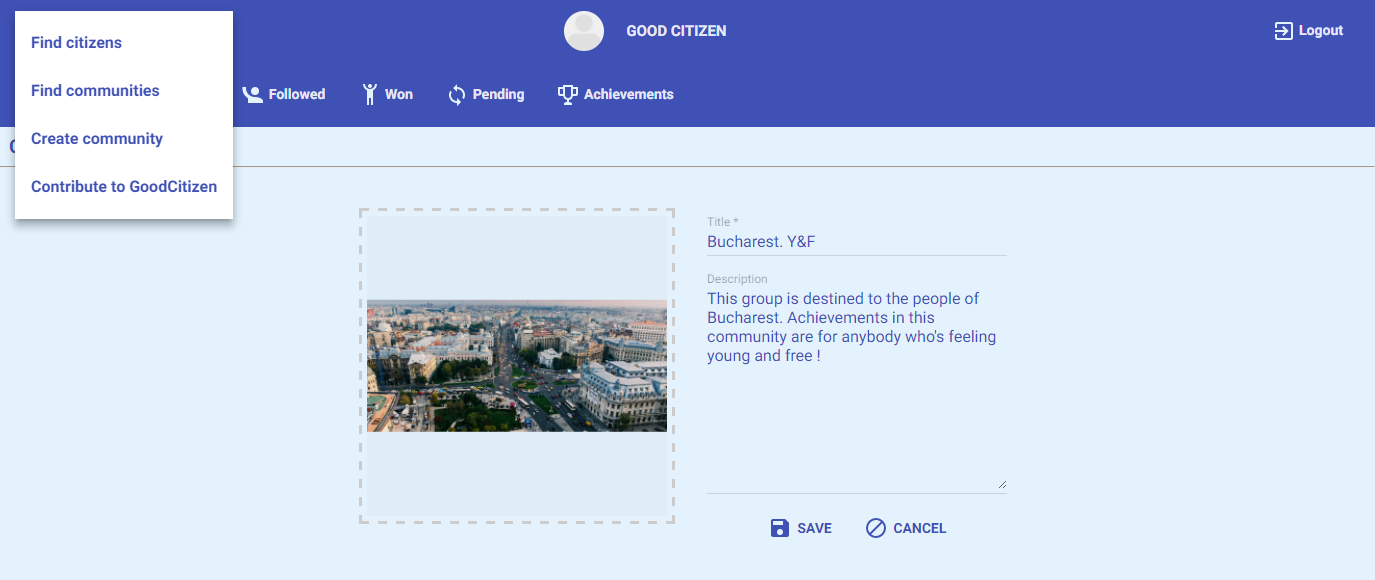
\includegraphics[width=\textwidth,height=\textheight,keepaspectratio]{create-community.png}
    % 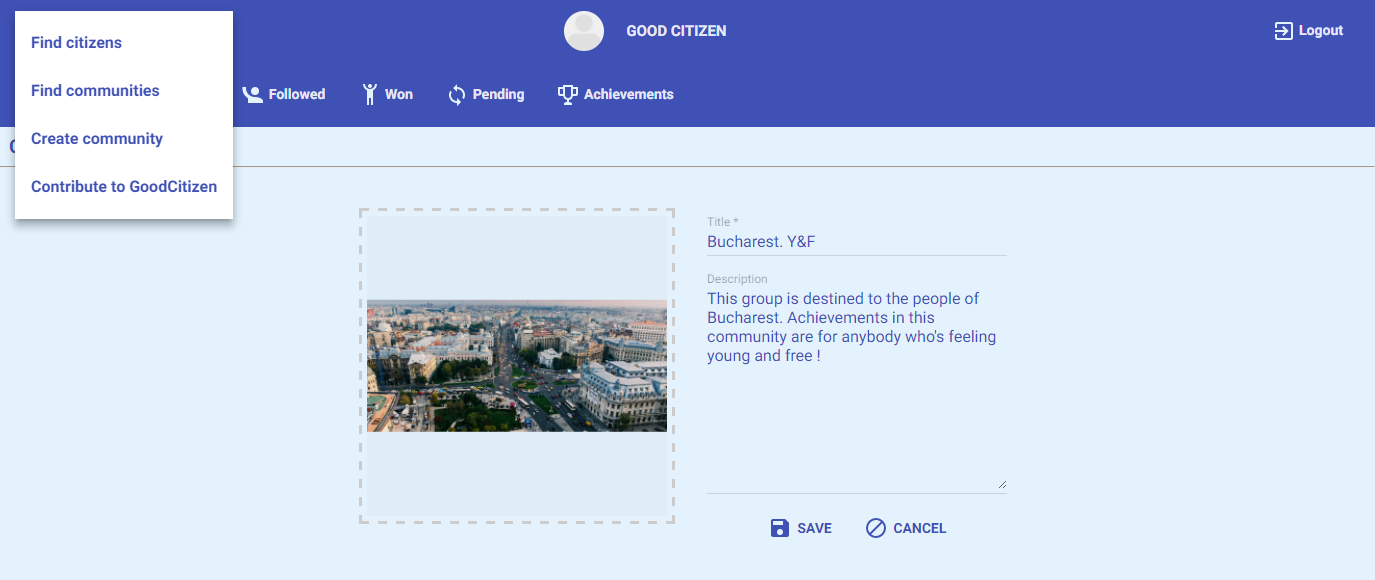
\includegraphics[height=0.43\linewidth]{create-community.png}
    \centering
    \caption{Crearea unei comunități.}
    \label{fig:create-community}
    \end{figure}        
\subsection{Extinderea rețelei de socializare}
    O rețea de socializare se extinde în funcție de feedback-ul primit de la utilizatori. Aplicația 
    „GoodCitizen” dispune de un formular de feedback (Fig.~\ref{fig:feedback}) pentru utilizatori, unde aceștia pot semnala erori 
    și propune noi funcționalități. Dacă propunerile sunt relevante și sugerate de mai mulți utilizatori acestea 
    vor putea fi adăugate în aplicație. 
    \begin{figure}[h]
    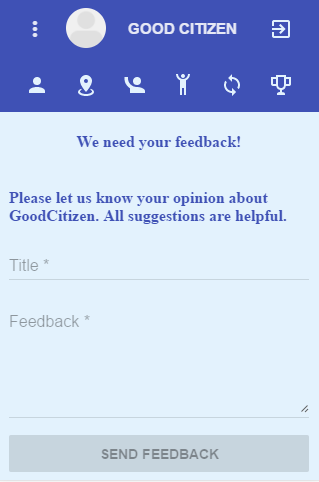
\includegraphics[height=0.4\linewidth]{feedback.png}
    \centering
    \caption{Formularul de feedback.}
    \label{fig:feedback}
    \end{figure}   

\section{Diagrame}
\subsection{Diagrame UML use-case}
    În acest subcapitol sunt prezentate patru diagrame de tip use-case: procesul de
înregistrare/autentificare, funcționalitățile disponibile utilizatorul,
diagrama drepturilor într-o comunitate și diagrama cu drepturile creatorului/administratorului.
în contul personal:
    \begin{figure}[h]
    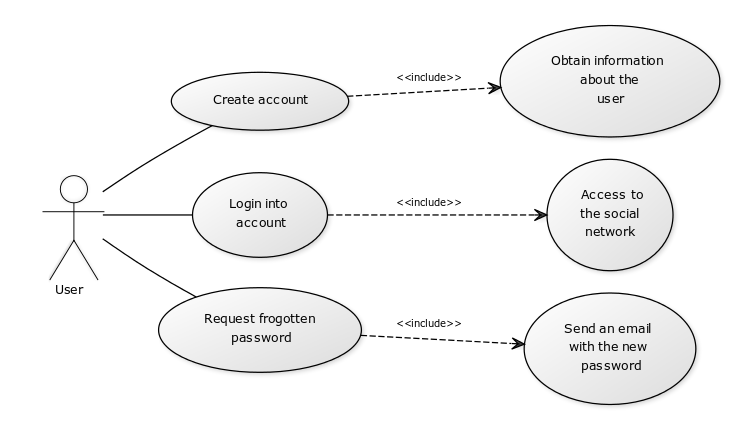
\includegraphics[width=\textwidth,height=\textheight,keepaspectratio]{use-case1.png}
    % 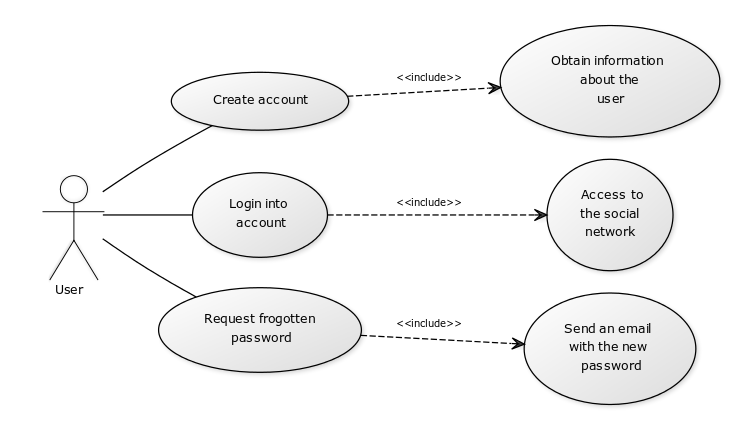
\includegraphics[height=0.6\linewidth]{use-case1.png}
    \centering
    \caption{Diagrama use-case aferentă procesului de înregistrare/autentificare în aplicație.}
    \label{fig:use-case1}
    \end{figure}
    \begin{figure}[h]
    
\includegraphics[width=\textwidth,height=\textheight,keepaspectratio]{use-case3.png}
    % 
\includegraphics[height=0.4\linewidth]{use-case3.png}
    \centering
    \caption{Diagramă use-case aferentă drepturilor într-o comunitate ale unui utilizator.}
    \label{fig:use-case3}
    \end{figure} 
    \begin{figure}[h]
    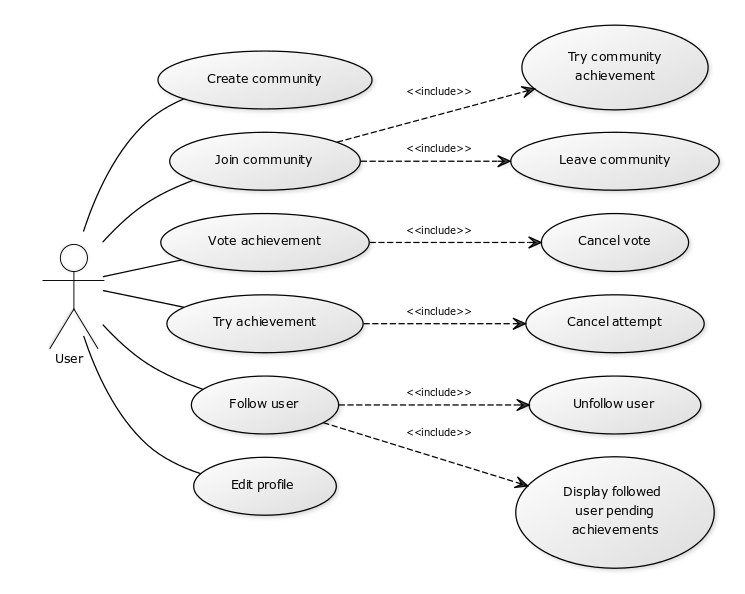
\includegraphics[width=\textwidth,height=\textheight,keepaspectratio]{use-case2.png}
    % 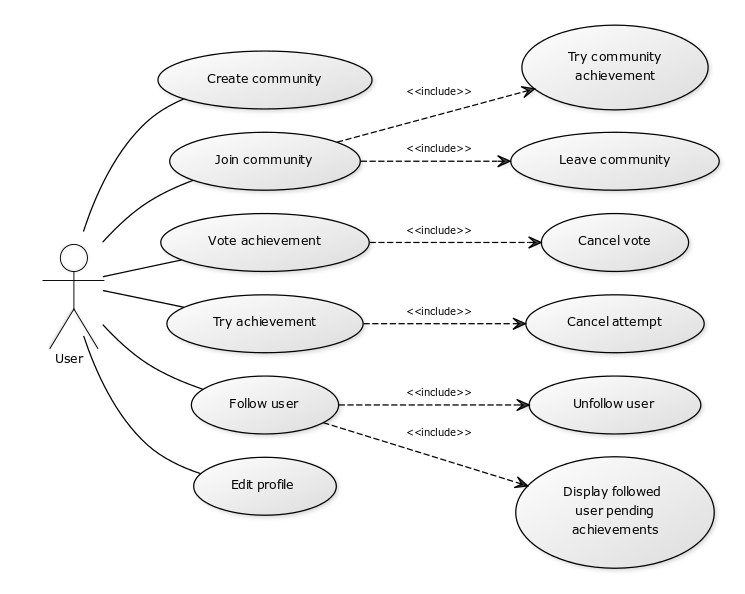
\includegraphics[height=0.7\linewidth]{use-case2.png}
    \centering
    \caption{Diagramă use-case aferentă funcționalităților unui utilizator}
    \label{fig:use-case2}
    \end{figure}    
    \begin{figure}[h]
    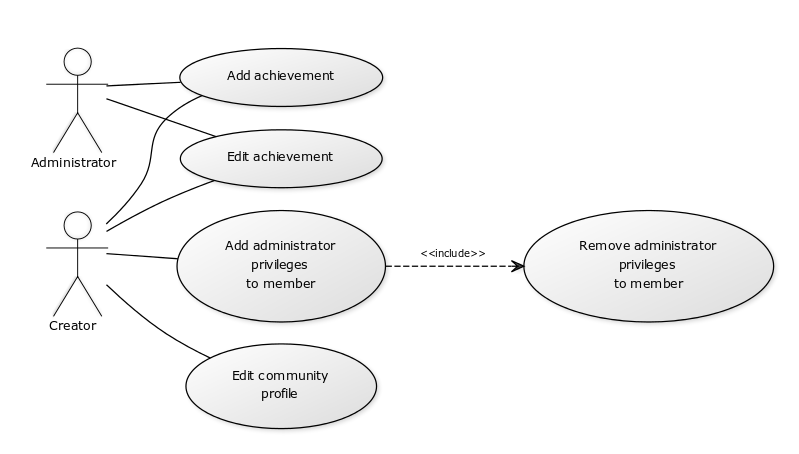
\includegraphics[width=\textwidth,height=\textheight,keepaspectratio]{use-case4.png}
    % 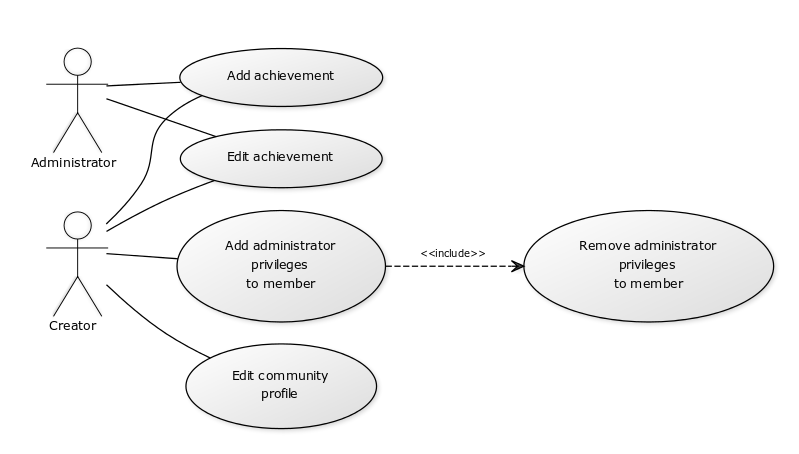
\includegraphics[height=0.5\linewidth]{use-case4.png}
    \centering
    \caption{Diagramă use-case aferentă drepturilor creatorului și administratorului într-o comunitate.}
    \label{fig:use-case4}
    \end{figure}
    \clearpage    
\subsection{Diagrama ER a bazei de date}
    Figura de mai jos(Fig.~\ref{fig:feedback}) reprezintă diagrama ER a bazei de date folosite de rețeaua de 
    socializare „GoodCitizen”.
    Entitățile \textit{CITIZEN, COMMUNITY, CATEGORY, ACHIEVEMENT și ROLE} sunt tabele ce conțin date
    despre cetățeni, comunități, realizări, categori de realizări și rolurile în aplicație ale unui utilizator.
    În tabela ROLE sunt inserate rolurile posibile ale unui utilizator în aplicație. În 
    implementarea actuală a aplicației este folosit un singur rol("USER"). În cazul extinderi 
    rețelei de socializare se pot adăuga roluri adiționale pentru alte tipuri de acces în aplicație.
    Entitățile \textit{USER\_ROLE, CITIZEN\_RELATION, CITIZEN\_COMMUNITY, CITIZEN\_ACHIEVEMENT și VOTE}
    sunt tabele de joncțiune formate datorită 
    relațiilor \textit{N la N}. 

    \begin{figure}[h]
    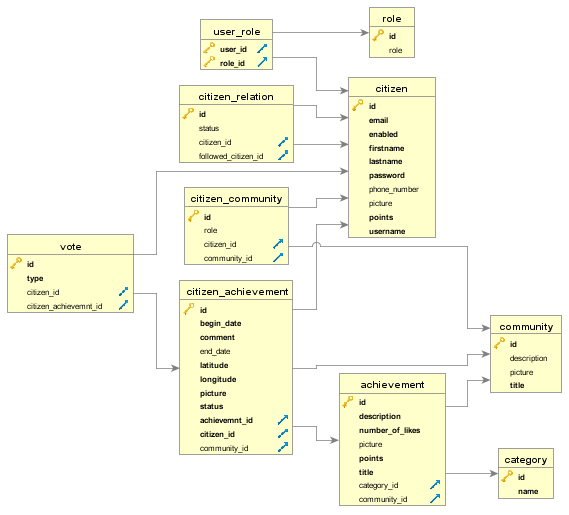
\includegraphics[width=\textwidth,height=\textheight,keepaspectratio]{er.png}
    % 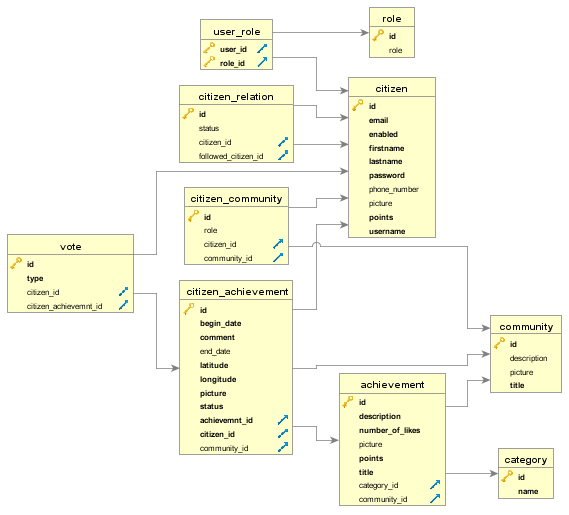
\includegraphics[height=0.95\linewidth]{er.png}
    \centering
    \caption{Diagramă ER a bazei de date.}
    \label{fig:er}
    \end{figure}    